\chapter{Requirements and Analysis}
\label{chapterlabel3}


This Chapter establishes the requirements and analysis for this work. The developments of the requirements is a crucial part of the analysis for almost all of the software development projects.

This phase is extremely useful, as for it's flexibility - if things that are unnecessarily complicated are discovered, or are less important to the client, they can be disregarded  or their importance could be downgraded so that they take less time. This is significantly useful for the implementation phase. This is also the easiest time to communicate with the client, while the subject matter is strictly textual, so any major issues or changes to the specifications can be established here.


\section{Problem Statement}
\label{problem_st}

Design a web based application, that allows surgeons to register an operation, upload and view all the extracted data coming from the operating theatre's sensors.


\section{Software Requirement Listing and Prioritization}
\label{sec:softreqlistandprior} 

This stage facilitates a comprehensive understanding of the client's needs and to appreciate the potential complexity of the system. Subsection \ref{sub:functional_req} details the functional requirements of our system.  Functional requirements show the behaviours of the system - what the client wants the system to do.  Subsection \ref{sub:non_functional_req} goes through the non-functional requirements, which affect the system's performance . 
The requirements were gathered through discussion with the client and also by continually iterating over what the application would be used for, so that additional focus should be given on the user needs.


 As mentioned, the requirements have been divided into functional and non-functional \cite{Software_Requirements}. They have also been prioritised according to the MoSCoW prioritisation technique\cite{cleggbarker1994}, in order to guide the progress of the project and to ensure that a base-level application that achieved the goals of the project. The MoSCoW priorities refer to the order of design and development in order. Must have, Should Have, Could Have, and Won't have requirements.




\subsection{Functional Requirements}
\label{sub:functional_req}

\newcounter{magicrownumbers}
\newcommand\rownumber{\stepcounter{magicrownumbers}\arabic{magicrownumbers}}
{
\footnotesize
%\centering
\begin{longtable}{|p{0.5cm}|p{13cm}p{1.3cm}|}

\rowcolor[HTML]{000000}
{\color[HTML]{FFFFFF} \textbf{ID}} & {\color[HTML]{FFFFFF} \textbf{Functional Requirements}}  & {\color[HTML]{FFFFFF} \textbf{Priority}} \\ \hline \endhead
\multicolumn{3}{|c|}{\textbf{Uploading a new Operation}} \\ \hline
\rownumber & The platform shall support a User Interface that will allow the user to register a new operation &Must  \\ \hline
\rownumber & The platform shall be able to take as input from the user, the hospital that the operation took place &Must  \\ \hline
\rownumber & The platform shall be able to take as input from the user, the operating room that the operation took place &Must  \\ \hline
\rownumber & The platform shall be able to take as input from the user, all the staff that participated in the operation &Must  \\ \hline
\rownumber & The platform shall be able to take as input from the user, the type of the operation (Neurosurgery, Hand surgery, Paediatric surgery etc.) &Must  \\ \hline
\rownumber & The platform shall be able to take as input from the user, the specific patient that has undergone the surgery including the patients unique identification number &Must  \\ \hline
\rownumber & The platform shall be able to take as input from the user, all the video files that were produced during the operation &Must  \\ \hline
\rownumber & The platform shall be able to take as input from the user, all the audio files that were produced during the operation &Must  \\ \hline
\rownumber & The platform shall be able to take as input from the user, the file extracted from the patient's monitoring system &Should  \\ \hline
\rownumber & The platform shall be able to record, store and distinguish data from different operating theatres &Must  \\ \hline
\rownumber & The platform shall be able to store all the input data from the user to a relational database &Must  \\ \hline
\rownumber & The platform shall store all the data coming from an operation in a way that all relevant data of the operation could be extracted &Must  \\ \hline
\rownumber & The platform shall be able to process the video, audio and patients monitoring files uploaded from the user &Must  \\ \hline
\rownumber & The platform shall be able to extract all the meta-data from the input files (encoded date, size, duration, file type, file name, full file path) &Must  \\ \hline
\rownumber & The platform shall be able to store the meta-data extracted from the input files, to the relational database &Must  \\ \hline
\rownumber & The platform shall be able to store the input files to an Azure Blob Storage Account &Must  \\ \hline
\rownumber & The platform shall be able to link the files stored in the Azure Blob Storage with the relative operation identification number stored in the relational database &Must  \\ \hline


\multicolumn{3}{|c|}{\textbf{Searching for an Operation}} \\ \hline
\rownumber & The platform shall support searching capabilities; the user of the platform must be able to search an operation/procedure using relevant criteria  &Must  \\ \hline
\rownumber & The platform shall support filtering capabilities where the user can apply specific filters for an operation (hospital name, operating room number, from/to date, doctors name, patient's name, type) &Must  \\ \hline

\multicolumn{3}{|c|}{\textbf{Details of an Operation}} \\ \hline
\rownumber & The platform shall be able to display a specific page where the user can see all the relative information and details of a specific operation &Must  \\ \hline
\rownumber & The platform shall be able to retrieve all the relevant data from the operation (video data, microphone data, patient's monitoring system data etc.) &Must  \\ \hline
\rownumber & The platform shall be able to convert the data coming from the different sensors to easily handled format ( e.g. convert a variety of video input to .avi) &Could  \\ \hline
\rownumber & The platform shall support the capability of switching to a specific moment in time and view all the recorded data at that moment &Could  \\ \hline
\rownumber & The platform shall be able to present to the user all the data recorded from the sensors at the same time. For example it could be able to view the panoramic camera, the light camera, the heart rate, the temperature of the room through the common factor of time. &Could  \\ \hline
\rownumber & The platform shall provide the media files' URL to the user in order for the user to have access to them and re-play them &Must  \\ \hline

\caption[Functional Requirements]{Functional Requirements} % needs to go inside longtable environment
\label{functionalreq}
\end{longtable}
}

\subsection{Non Functional Requirements}
\label{sub:non_functional_req}

{\footnotesize
%\newcommand\rownumber{\stepcounter{magicrownumbers}\arabic{magicrownumbers}}
%\centering
\begin{longtable}{|p{0.5cm}|p{13cm}p{1.3cm}|}

\rowcolor[HTML]{000000}
{\color[HTML]{FFFFFF} \textbf{ID}} &{\color[HTML]{FFFFFF} \textbf{Non-Functional Requirements}}  & {\color[HTML]{FFFFFF} \textbf{Priority}} \\ \hline \endhead
\rownumber & The platform shall use web browser as its user interface & Must \\ \hline
\rownumber & The platform shall support new sensor adding or should require minimal work for new, unknown sensor adding & Should \\ \hline
\rownumber & The platform shall store all the input data in a way that they could be extracted for machine learning purposes (machine learn-able data) & Must \\ \hline
\rownumber & The platform shall be independent of the format of the input data & Should  \\ \hline
\rownumber & The platform shall work on a wide range of operating conditions (screen size, internet connection, performance) & Must \\ \hline
\rownumber & The platform shall be a C\# web application with an MySQL Database & Should \\ \hline
\rownumber & The System shall present search results within 5 seconds & Should \\ \hline

\caption[Non-Functional Requirements]{Non-Functional Requirements} % needs to go inside longtable environment
\label{nonfunctionalreq}
\end{longtable}
}


\section{Domain Modelling}
\label{sec:DomainModelling}
The domain model looks to identify the objects of a system in terms of the requirements. It provides a conceptual real-world view of the system and enables a simplistic overview of the system's functionalities in terms of the problem domain entities \cite{DomainModeling}.
More specifically, the classes were derived from the requirements list where the identified entities were marked in bold. Therefore, it is now possible to create a simple draft domain model from these entities. Furthermore, objects which were deemed redundant from this iteration were also
discarded to refine the list of entities. This initial model was then revised and additional domain objects were
added. Similar to previous analyses, the domain model is therefore the result of an iterative process.

Following the refinement process, using the identified entities of the requirements list, the domain model was revised in order to find any unspotted domain entities that weren't already in the requirements list. 
Figure \ref{domain_model} shows the model that resulted after the various iterations. It is a summary of the responsibilities of the system on a general level and was the basis for constructing the use cases in subsection \ref{sub:use_case_analysis}.

\begin{figure}[h]
\begin{center}
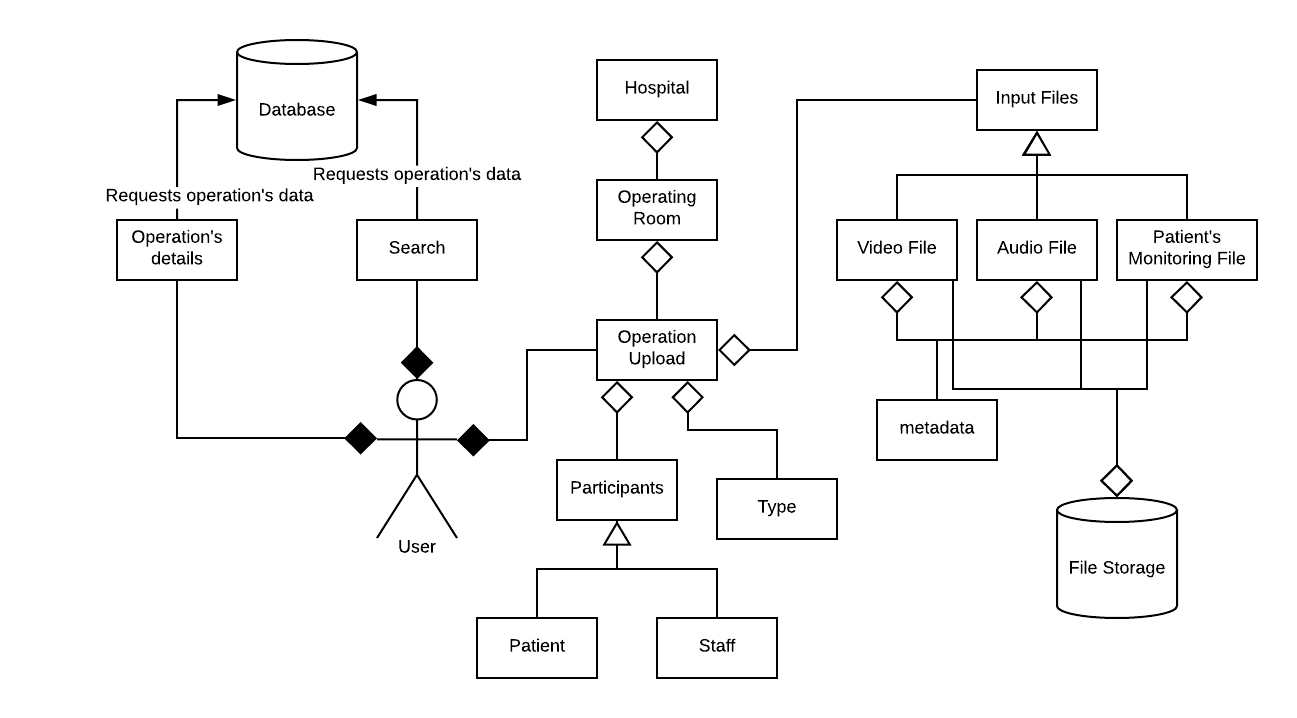
\includegraphics[width=17cm]{imgs/Domain_Model.png}
\end{center}\vspace{-0.3cm}
\caption[Domain Model]{Conceptual model of the system's problem domain} \label{domain_model}
\end{figure}



\section{Use Case Analysis}
\label{sub:use_case_analysis}

Following the domain modelling and the gathering of requirements analysed in sections \ref{sec:DomainModelling} and \ref{sec:softreqlistandprior} respectively, use cases were developed. The defined domain entities and requirements were used to construct the use cases and their basic relationships. The construction of the uses cases allows the solid organisation of the functional requirements of the project, in order to make sure that they meet the front-end requirements and also to make sure that they are fully encompassing. A use case describes a scenario where a user interacts with the application in order to achieve a specific outcome \cite{usecases3}. Use cases are described from the users point of view rather than a technical point of view. As such, use cases are very effective at visualising and communicating the final product to the client and incorporating the client's voice into the requirements of the project \cite{usecases2}.

A complete overview of the identified use cases is shown in  Table \ref{UC-Summary} and from Table \ref{UC01} to Table \ref{UC03}, all the detailed specification for each use case are shown. Each specification includes details of each use case,the main flows, error flows, post-conditions, pre-conditions and the trigger event.


\begin{table}[h]
\centering
\begin{tabular}{|
>{\columncolor[HTML]{C0C0C0}}p{1.5cm}|p{8cm}|}
\hline
\textbf{ID} & \cellcolor[HTML]{C0C0C0}\textbf{Use Case}  \\ \hline
UC01        & \textbf{Upload a new operation}                           \\ \hline
UC02        & \textbf{Search for an operation}                             \\ \hline
UC03        & \textbf{View operation detals}                                                         \\ \hline
\end{tabular}
\caption[Use Case Listing]{List of use cases}
\label{UC-Summary}
\end{table}


\begin{table}[h]
\footnotesize
\centering
\begin{tabular}{|
>{\columncolor[HTML]{C0C0C0}}p{2.7cm}|p{12cm}|}
\hline
Use Case          & Upload a new operation \\ \hline
ID                & UC01                                                                                                                                                                                                                                                                                          \\ \hline
Brief Description & The user wishes to register the operation to the System                                                                                                                                                                                                                         \\ \hline
Preconditions     & User must have all the necessary files and information of the operation                                                                                                                                                                                                                                         \\ \hline
Main Flow         & \begin{tabular}[c]{@{}l@{}}1. Home page is displayed\\ 2. The User selects to register a new operation\\ 3. The User enters the hospital name \\ 4. The User enters the operating room number \\ 5. The User enters all the staff that participated in the operation\\6. The User enters the patient that underwent the surgery\\ 7. The User enters the type of the operation\\ 8. The User selects all the relevant video files \\9. The User selects all the relevant audio files \\10. The User selects the patient's monitoring file \end{tabular}                                                                      \\ \hline
Post Conditions   & A new operation has been registered to the database and the files have been uploaded to the file storage                                                                                                                                                                                                                                                        \\ \hline
Alternative Flows & The User no longer wishes to upload yet the operation to the System and cancels the registration of the operation                                                                                                                                                                                                        \\ \hline
Error Flow        & \begin{tabular}[c]{@{}l@{}}1. The User does not enter any of the 1-7 fields and at least one input file \\ 2. An error message is displayed \end{tabular} \\ \hline
Trigger Event     & The user chooses to add new operation \\ \hline
\end{tabular}
\caption[Use Case 01 - Upload a new operation]{Use Case 01 - Upload a new operation}
\label{UC01}
\end{table}


\begin{table}[h]
\footnotesize
\centering
\begin{tabular}{|
>{\columncolor[HTML]{C0C0C0}}p{2.7cm}|p{12cm}|}
\hline
Use Case          & Search for an operation \\ \hline
ID                & UC02                                                                                                                                                                                                                                                                                          \\ \hline
Brief Description & The User wishes to find an operation from the database \\ \hline
Preconditions     & At least one operation must have been registered to the system \\ \hline
Main Flow         & \begin{tabular}[c]{@{}l@{}}1. Home page is displayed\\ 2. The 20 most recent uploaded operations are displayed\\ 3. The User uses the Filters to input hospital name,operating room number,\\ from/to date and participated staff  \\ 4. The filtered results are displayed, ordered by date (from most recent to oldest) \end{tabular}                                                                      \\ \hline
Post Conditions   & The User can see the Operations that correspond to the Filters they have applied \\ \hline
Alternative Flows & The Operation that the User searches for and the Filters applied produce no results \\ \hline
Error Flow        &  None \\ \hline
Trigger Event     & The User wishes to Search for an Operation \\ \hline
\end{tabular}
\caption[Use Case 02 - Search for an operation]{Use Case 02 - Search for an operation}
\label{UC02}
\end{table}


\begin{table}[h]
\footnotesize
\centering
\begin{tabular}{|
>{\columncolor[HTML]{C0C0C0}}p{2.7cm}|p{12cm}|}
\hline
Use Case          & View operation details \\ \hline
ID                & UC03 \\ \hline
Brief Description & The User can view the details of an Operation \\ \hline
Preconditions    & \begin{tabular}[c]{@{}l@{}}1. At least one operation must have been registered\\ 2. The User must have searched for an Operation\\  \end{tabular}                                                                      \\ \hline
Main Flow         & \begin{tabular}[c]{@{}l@{}}1. Home page is displayed\\ 2. The User searches for an Operation\\ 3. The User views the filtered results  \\ 4. The User selects the desired Operation \\ 5.The User views the Operation details \end{tabular}                                                                      \\ \hline
Post Conditions   & The Operation details are displayed to the User \\ \hline
Alternative Flows & The User does not wish to view the Operation details and so goes back to the homepage \\ \hline
Error Flow        &  System fails to report Operation Details \\ \hline
Trigger Event     & The User wishes to view the details of a listed Operation \\ \hline
\end{tabular}
\caption[Use Case 03 - View operation details]{Use Case 03 - View operation details}
\label{UC03}
\end{table}


\section{Use Case Diagram}
\label{sub:use_case_diagram}


The use case diagram which is depicted in Figure \ref{UC-diagram} is derived from the use case Listing which is basic foundation for the creation of the use case diagram.


\begin{figure}[h]
\begin{center}
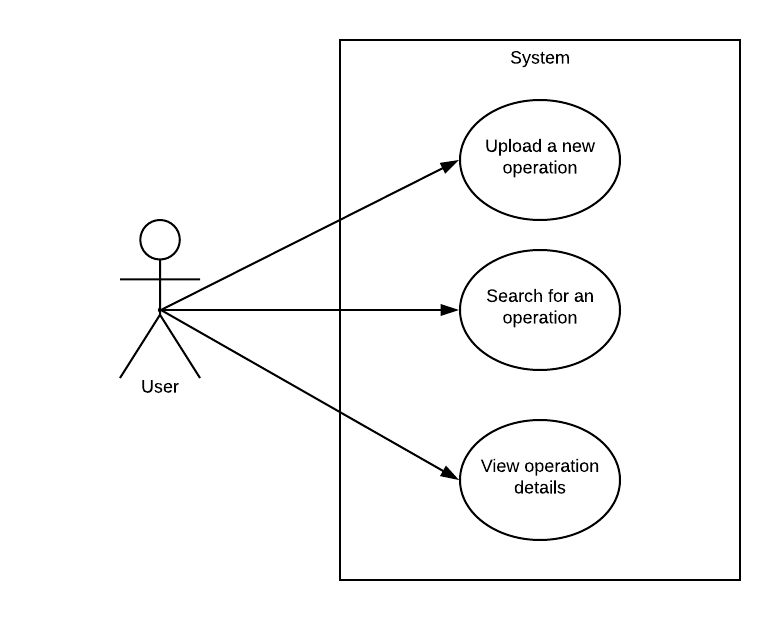
\includegraphics[width=17cm]{imgs/Use_Case_Diagram.png}
\end{center}\vspace{-0.3cm}
\caption[Use Case Diagram]{Use case diagram} \label{UC-diagram}
\end{figure}


\section{Object Oriented Analysis}
\label{sub:object_oriented_analysis}

% This just dumps some pseudolatin in so you can see some text in place.


\blindtext
\blindtext

